%%%%%%%%%%%%%%%%%%%%%%%%%%%%%%%%%%%
%This is the LaTeX COMMUNICATION template for RSC journals
%Copyright The Royal Society of Chemistry 2016
%%%%%%%%%%%%%%%%%%%%%%%%%%%%%%%%%%%

\documentclass[twoside,twocolumn,9pt]{article}
\usepackage{extsizes}
\usepackage[super,sort&compress,comma]{natbib} 
\usepackage[version=3]{mhchem}
\usepackage[left=1.5cm, right=1.5cm, top=1.785cm, bottom=2.0cm]{geometry}
\usepackage{balance}
\usepackage{mathptmx}
\usepackage{sectsty}
\usepackage{graphicx} 
\usepackage{lastpage}
\usepackage[format=plain,justification=justified,singlelinecheck=false,font={stretch=1.125,small,sf},labelfont=bf,labelsep=space]{caption}
\usepackage{float}
\usepackage{fancyhdr}
\usepackage{fnpos}
\usepackage[english]{babel}
\addto{\captionsenglish}{%
  \renewcommand{\refname}{Notes and references}
}
\usepackage{array}
\usepackage{droidsans}
\usepackage{charter}
\usepackage[T1]{fontenc}
\usepackage[usenames,dvipsnames]{xcolor}
\usepackage{setspace}
\usepackage[compact]{titlesec}
\usepackage{hyperref}
%%%Please don't disable any packages in the preamble, as this may cause the template to display incorrectly.%%%


\usepackage{epstopdf}%This line makes .eps figures into .pdf - please comment out if not required.

\definecolor{cream}{RGB}{222,217,201}

\begin{document}

\pagestyle{fancy}
\thispagestyle{plain}
\fancypagestyle{plain}{
%%%HEADER%%%
\renewcommand{\headrulewidth}{0pt}
}
%%%END OF HEADER%%%

%%%PAGE SETUP - Please do not change any commands within this section%%%
\makeFNbottom
\makeatletter
\renewcommand\LARGE{\@setfontsize\LARGE{15pt}{17}}
\renewcommand\Large{\@setfontsize\Large{12pt}{14}}
\renewcommand\large{\@setfontsize\large{10pt}{12}}
\renewcommand\footnotesize{\@setfontsize\footnotesize{7pt}{10}}
\renewcommand\scriptsize{\@setfontsize\scriptsize{7pt}{7}}
\makeatother

\renewcommand{\thefootnote}{\fnsymbol{footnote}}
\renewcommand\footnoterule{\vspace*{1pt}% 
\color{cream}\hrule width 3.5in height 0.4pt \color{black} \vspace*{5pt}} 
\setcounter{secnumdepth}{5}

\makeatletter 
\renewcommand\@biblabel[1]{#1}            
\renewcommand\@makefntext[1]% 
{\noindent\makebox[0pt][r]{\@thefnmark\,}#1}
\makeatother 
\renewcommand{\figurename}{\small{Fig.}~}
\sectionfont{\sffamily\Large}
\subsectionfont{\normalsize}
\subsubsectionfont{\bf}
\setstretch{1.125} %In particular, please do not alter this line.
\setlength{\skip\footins}{0.8cm}
\setlength{\footnotesep}{0.25cm}
\setlength{\jot}{10pt}
\titlespacing*{\section}{0pt}{4pt}{4pt}
\titlespacing*{\subsection}{0pt}{15pt}{1pt}
%%%END OF PAGE SETUP%%%

%%%FOOTER%%%
\fancyfoot{}
\fancyfoot[LO,RE]{\vspace{-7.1pt}
\includegraphics[height=9pt]{head_foot/LF}}
\fancyfoot[CO]{\vspace{-7.1pt}\hspace{13.2cm}
\includegraphics{head_foot/RF}}
\fancyfoot[CE]{\vspace{-7.2pt}\hspace{-14.2cm}
\includegraphics{head_foot/RF}}
\fancyfoot[RO]{\footnotesize{\sffamily{1--\pageref{LastPage} ~\textbar  \hspace{2pt}\thepage}}}
\fancyfoot[LE]{\footnotesize{\sffamily{\thepage~\textbar\hspace{3.45cm} 1--\pageref{LastPage}}}}
\fancyhead{}
\renewcommand{\headrulewidth}{0pt} 
\renewcommand{\footrulewidth}{0pt}
\setlength{\arrayrulewidth}{1pt}
\setlength{\columnsep}{6.5mm}
\setlength\bibsep{1pt}
%%%END OF FOOTER%%%

%%%FIGURE SETUP - please do not change any commands within this section%%%
\makeatletter 
\newlength{\figrulesep} 
\setlength{\figrulesep}{0.5\textfloatsep} 

\newcommand{\topfigrule}{\vspace*{-1pt}% 
\noindent{\color{cream}\rule[-\figrulesep]{\columnwidth}{1.5pt}} }

\newcommand{\botfigrule}{\vspace*{-2pt}% 
\noindent{\color{cream}\rule[\figrulesep]{\columnwidth}{1.5pt}} }

\newcommand{\dblfigrule}{\vspace*{-1pt}% 
\noindent{\color{cream}\rule[-\figrulesep]{\textwidth}{1.5pt}} }

\makeatother
%%%END OF FIGURE SETUP%%%

%%%TITLE AND AUTHORS%%%
\twocolumn[
  \begin{@twocolumnfalse}
{
\includegraphics[height=30pt]{head_foot/journal_name}\hfill\raisebox{0pt}[0pt][0pt]{
\includegraphics[height=55pt]{head_foot/RSC_LOGO_CMYK}}\\[1ex]

\includegraphics[width=18.5cm]{head_foot/header_bar}}\par
\vspace{1em}
\sffamily
\begin{tabular}{m{4.5cm} p{13.5cm} }


\includegraphics{head_foot/DOI} & \noindent\LARGE{\textbf{Discovery of SARS-CoV-2 main protease inhibitors using a synthesis-directed \emph{de novo} design model $^\dag$}} \\%Article title goes here instead of the text "This is the title"
 & \vspace{0.3cm} \\

 & \noindent\large{Aaron Morris,\textit{$^{a \ddag}$} William McCorkindale \textit{$^{b\ddag}$}, The COVID Moonshot Consortium \textit{$^{c}$}, Nir Drayman \textit{$^{d}$}, John D. Chodera \textit{$^{e}$}, Sava\c{s} Tay \textit{$^{d}$}, Nir London \textit{$^{f}$}, and Alpha A. Lee\textit{$^{a \P}$}} \\%Author names go here instead of "Full name", etc.

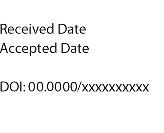
\includegraphics{head_foot/dates} & \\

\end{tabular}

 \end{@twocolumnfalse} \vspace{0.6cm}

  ]
%%%END OF TITLE AND AUTHORS%%%

%%%FONT SETUP - please do not change any commands within this section
\renewcommand*\rmdefault{bch}\normalfont\upshape
\rmfamily
\section*{}
\vspace{-1cm}


%%%FOOTNOTES%%%

\footnotetext{\textit{$^{a}$~PostEra Inc, 2 Embarcadero Centre, San Franciso, CA 94111, United States of America}}
\footnotetext{\textit{$^{b}$~Department of Physics, University of Cambridge, CB3 0HE, United Kingdom }}
\footnotetext{\textit{$^{c}$~The COVID Moonshot Consortium, \url{www.postera.ai/covid} }}
\footnotetext{\textit{$^{d}$~The Pritzker School for Molecular Engineering, The University of Chicago, Chicago, IL, USA }}
\footnotetext{\textit{$^{e}$~Computational and Systems Biology Program Sloan Kettering Institute, Memorial Sloan Kettering Cancer Center, New York, NY 10065, USA }}
\footnotetext{\textit{$^{f}$~Department of Organic Chemistry, The Weizmann Institute of Science, 76100, Rehovot, Israel }}

%Please use \dag to cite the ESI in the main text of the article.
%If you article does not have ESI please remove the the \dag symbol from the title and the footnotetext below.
\footnotetext{\dag~Electronic Supplementary Information (ESI) contains experimental and assay details. Our training set, de novo design method and generated molecules are available on \url{https://github.com/wjm41/mpro-rank-gen}.}
%additional addresses can be cited as above using the lower-case letters, c, d, e... If all authors are from the same address, no letter is required

\footnotetext{\ddag~These authors contributed equally to this work. }
\footnotetext{\P E-mail: alpha.lee@postera.ai }

%%%END OF FOOTNOTES%%%

%%%ABSTRACT%%%%

\sffamily{\textbf{The SARS-CoV-2 main viral protease ($\mathrm{M}^\mathrm{pro}$) is an attractive target for antivirals given its distinctiveness from host proteases, essentiality in the viral life cycle and conservation across coronaviridae. We launched the COVID Moonshot initiative to rapidly develop patent-free antivirals with open science and open data. Here we report the use of machine learning for \emph{de novo} design, coupled with synthesis route prediction, in our campaign. We discover novel chemical scaffolds active in biochemical and live virus assays, synthesized with model generated routes. }}\\

%The abstrast goes here instead of the text "The abstract should be..."

%%%END OF ABSTRACT%%%%

\rmfamily %Please do not remove this line.

%%%MAIN TEXT%%%%

%Intro to COVID19 and Moonshot

Coronaviruses are a family of pathogens that is frequently associated with serious and highly infectious human diseases, from the common cold to the SARS-CoV pandemic (2003, 774 deaths, 11\% fatality rate), MERS-CoV pandemic (2012, 858 deaths, 34\% fatality rate) and most recently the COVID-19 pandemic (ongoing pandemic, 1.7 million deaths up to Dec 2020). %However, to date there is no approved oral antiviral for coronavirus. 

The main protease ($\mathrm{M}^\mathrm{pro}$) is one of the best characterized drug targets for direct-acting antivirals \cite{pillaiyar2016overview,cannalire2020targeting}. $\mathrm{M}^\mathrm{pro}$ is essential for viral replication and its binding site is distinct from known human proteases, thus inhibitors are unlikely to be toxic \cite{jin2020structure,liu2020development}. Moreover, the high degree of conservation across different coronaviruses renders $\mathrm{M}^\mathrm{pro}$ targeting a fruitful avenue towards pan-cornavirus antivirals \cite{ullrich2020sars}. To date, most reported $\mathrm{M}^\mathrm{pro}$ inhibitors are peptidomimetics, covalent, or both \cite{cannalire2020targeting}. Peptidomimetics are challenging to develop into oral therapeutics, and covalent inhibitors incur additional idiosyncratic toxicity risks. We launched the COVID Moonshot consortium in March 2020, aiming to find oral antivirals against COVID-19 in an open-science, patent-free manner \cite{chodera2020crowdsourcing}. 

Here we report the prospective use of a simple model to rapidly expand hits. Starting from 42 compounds with $\mathrm{IC}_{50}$ within assay dynamic range ($<100 \mu$M) and 515 inactives, our model designed 5 new compounds predicted to have higher activity, together with predicted synthetic routes. All designs were were chemically synthesized and experimentally tested, and 3 have measurable activity against $\mathrm{M}^\mathrm{pro}$. The top compound has comparable $\mathrm{M}^\mathrm{pro}$ inhibition to the best in the training set, but with a different scaffold, and is active against the OC43 coronavirus in a live virus assay. 

%Describe GenChem 
Algorithmic \emph{de novo} design aims to automatically generate compounds that are chemically diverse, synthetically accessible and biologically active \cite{schneider2016novo}. Classic approaches apply heuristics to fragment and modify known active compounds, with the region of chemical space explored and synthetic accessibility constrained by those rules \cite{brown2004graph,patel2009knowledge,hartenfeller2012dogs}. Recent machine learning approaches explore chemical space in more abstract molecular representation space \cite{gomez2018automatic,segler2018generating}, but this often comes at the expense of synthetic accessibility \cite{gao2020synthesizability}. Our approach builds on rule-based fragmentation and molecule generation, but employs a method that combines regression and classification amid noisy data, and use of machine learning to predict synthesis routes. Our model comprises two parts: compound prioritisation and chemical space exploration. 

%describe ranking model + result 
Our compound prioritisation model aims to predict whether a designed compound is likely to be an improvement in activity over the incumbent. However, as is typical in the hit-expansion stage, bioactivity modelling is hindered by insufficient data where the majority of compounds are inactive, and noisy data as measurement variability increases for lower affinity compounds. Thresholding the data and framing the problem as classification of active/inactive would not allow us to rank compounds based on predicted improvement over the incumbent, yet the amount of measured bioactivity data and the measurement noise  makes a regression approach challenging.


To overcome both challenges, we develop a learning-to-rank framework \cite{duffy2010molecular,agarwal2010ranking}. Rather than training a regression model to predict the $\mathrm{IC}_{50}$ of a compound, we instead train a classifier to predict whether a compound is more or less active than another compound, with the input to the model being the \emph{difference} in molecular descriptors between the molecules (see Figure \ref{fig:roc_plot} for a schematic). This model accounts for both compounds with $\mathrm{IC}_{50}$ measurements and compounds that are simply inactive -- active compounds are ranked by their $\mathrm{IC}_{50}$, all inactives with no measurable $\mathrm{IC}_{50}$ are considered less active than active compounds, and inactive-inactive pairs are ignored. Further, we account for noise by only considering $\mathrm{IC}_{50}$ differences amongst actives above 5 $\mu M$. We use the FastAI Tabular model \cite{howard2018fastai}, with input features generated from concatenated Morgan, Atom Pair, and Topological Torsion fingerprints implemented in RDkit \cite{rdkit}, and dataset was randomly split into training (80\%) and testing (20\%); details about model implementation can be found in ESI and source code.


Figure \ref{fig:roc_plot} shows that our binary ranking model achieves an AUC of 0.88 (95\% CI: [0.83,0.96]) in ranking ligands within the test set, and AUC for 0.94 (95\% CI: [0.91,0.98]) where we compare a ligand in the training set against another ligand in the test set; the latter is more relevant as our goal is finding ligands more active than the best incumbent. The 95\% confidence interval is computed using bootstrapping. We also compare our model against OpenEye’s FRED hybrid docking mode as implemented in the ``Classic OEDocking'' floe, a physics-based docking algorithm, on the Orion online platform, which achieves AUC of 0.72; 95\% CI: [0.722,0.723] (see ESI for implementation details). Note that docking does not require ligand bioactivity as training data, thus is not a directly comparison to machine learning. In the Supplementary Material, we discuss that our model ranks ligands better than a model that directly learns $\mathrm{IC}_{50}$ (AUC = 0.86; 95\% CI: [0.71,0.95]). 

Beyond train-test split, model performance can be evaluated from a time-split. Five months have elapsed from the time we deployed our model to select compounds to writing up the manuscript. During that time, the COVID Moonshot Consortium (a team of expert medicinal chemists) has independently designed, synthesised and tested 356 compounds \cite{moonshot2020covid}, out of which 15\% were better than the top 2 compounds (having $\mathrm{IC}_{50}$ comparable within error) in our dataset. Table \ref{table:time_split} shows that our model has an enrichment factor of $\sim$2, i.e. if we rescore the 356 compounds synthesized by the medicinal chemistry team using our model, and pick the top 1\%-10\% percentile, the proportion of molecules that would be better than the top 2 compounds would be $\sim$2x higher than human selection. 

%From a set of binary ranking, we can accurately rank-order the active ligands (Figure XXXb), with a higher rank correlation than using the quantitative activity data alone. We use the average probability of a ligand being ranked higher than ligands in the training set as a proxy for overall rank.

\begin{figure}
\centering
    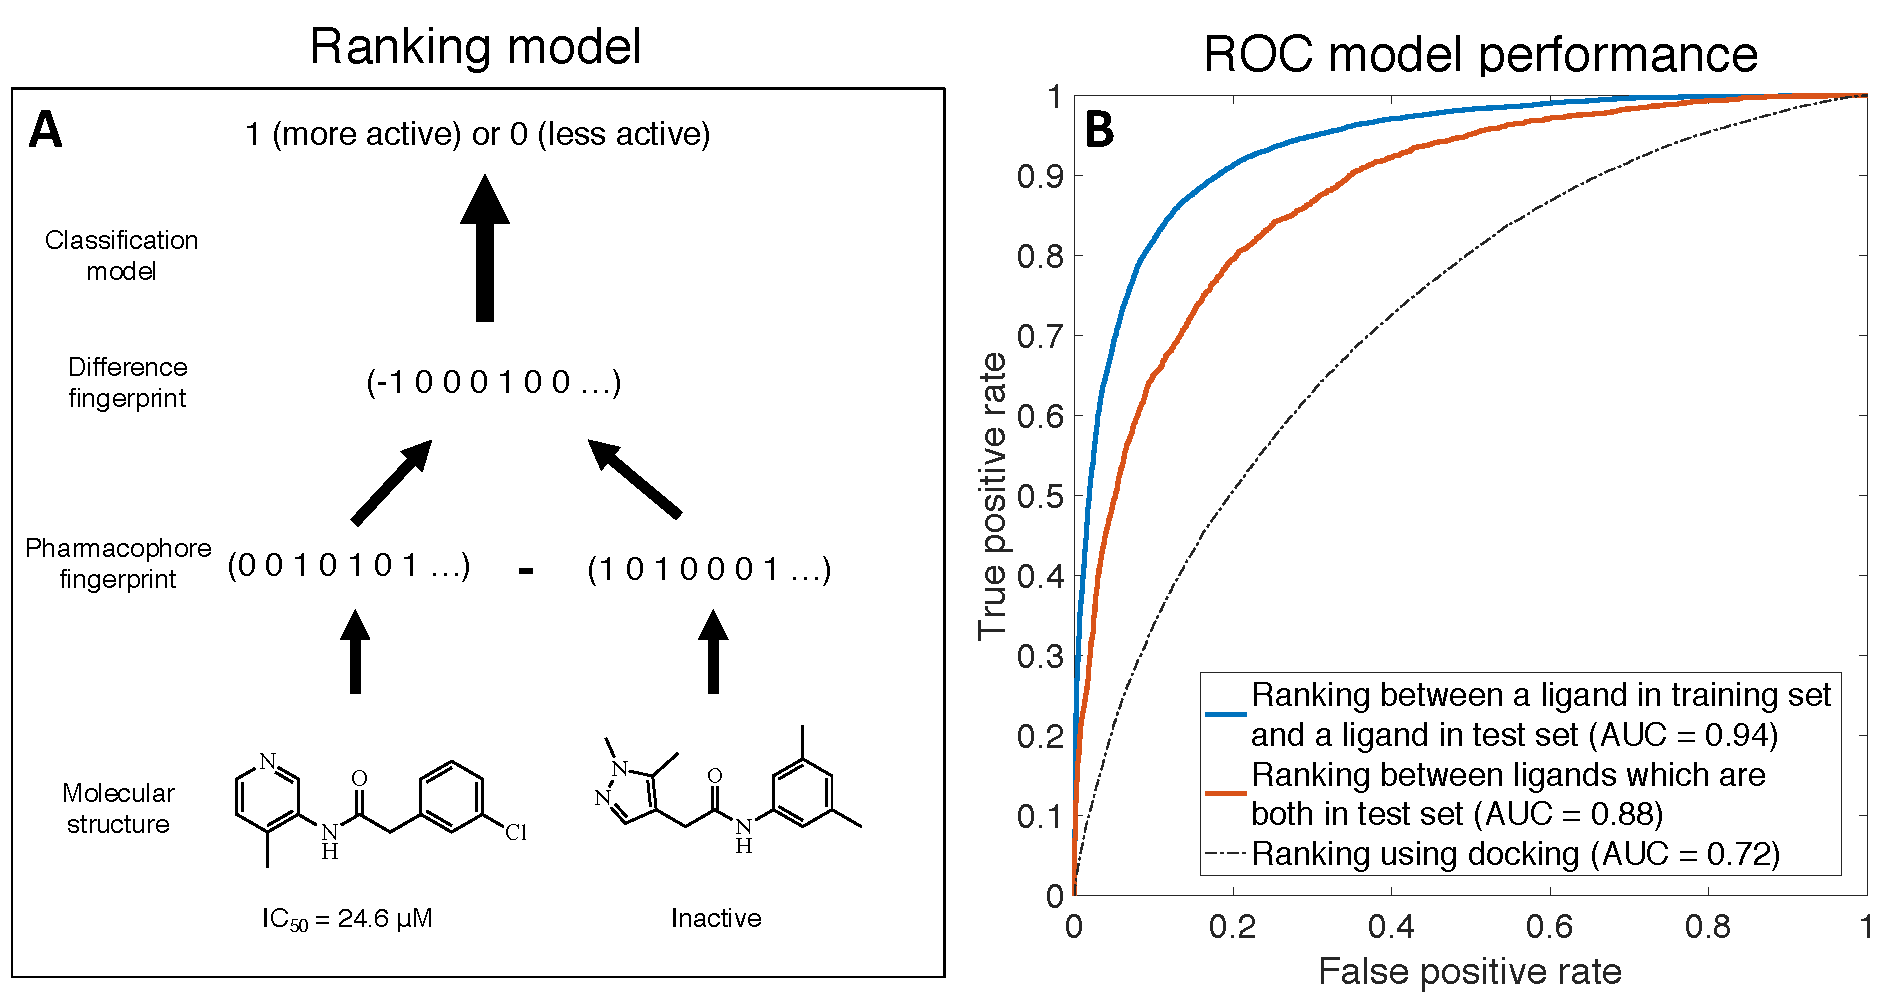
\includegraphics[scale=0.28]{ranking-model.pdf}
    \caption{Relative ranking of ligands can be predicted by our learning-to-rank machine learning model. (A) A schematic of the model setup. A classifier takes the difference in pharmacophore fingerprint between two molecules and predicts where one molecule is more or less active than the other. (B) The Receiver Operating Characteristic curve of classifying whether a molecule is more/less active than the other. AUC 95\% CI reported in main text.}
    \label{fig:roc_plot}
\end{figure}

\begin{table}
\centering
\begin{tabular}{|l|l|l|l|}
\hline
\textbf{Percentile}        & 1\% & 2.5\% & 10\% \\ \hline
\textbf{Enrichment Factor} & 1.7 & 2.3   & 1.7  \\ \hline
\end{tabular}
\caption{Enrichment factor for the time-split dataset, where we consider model performance on data arriving after the model has been deployed to generate compounds for synthesis and testing. }
\label{table:time_split}
\end{table}

\begin{figure}
\centering
         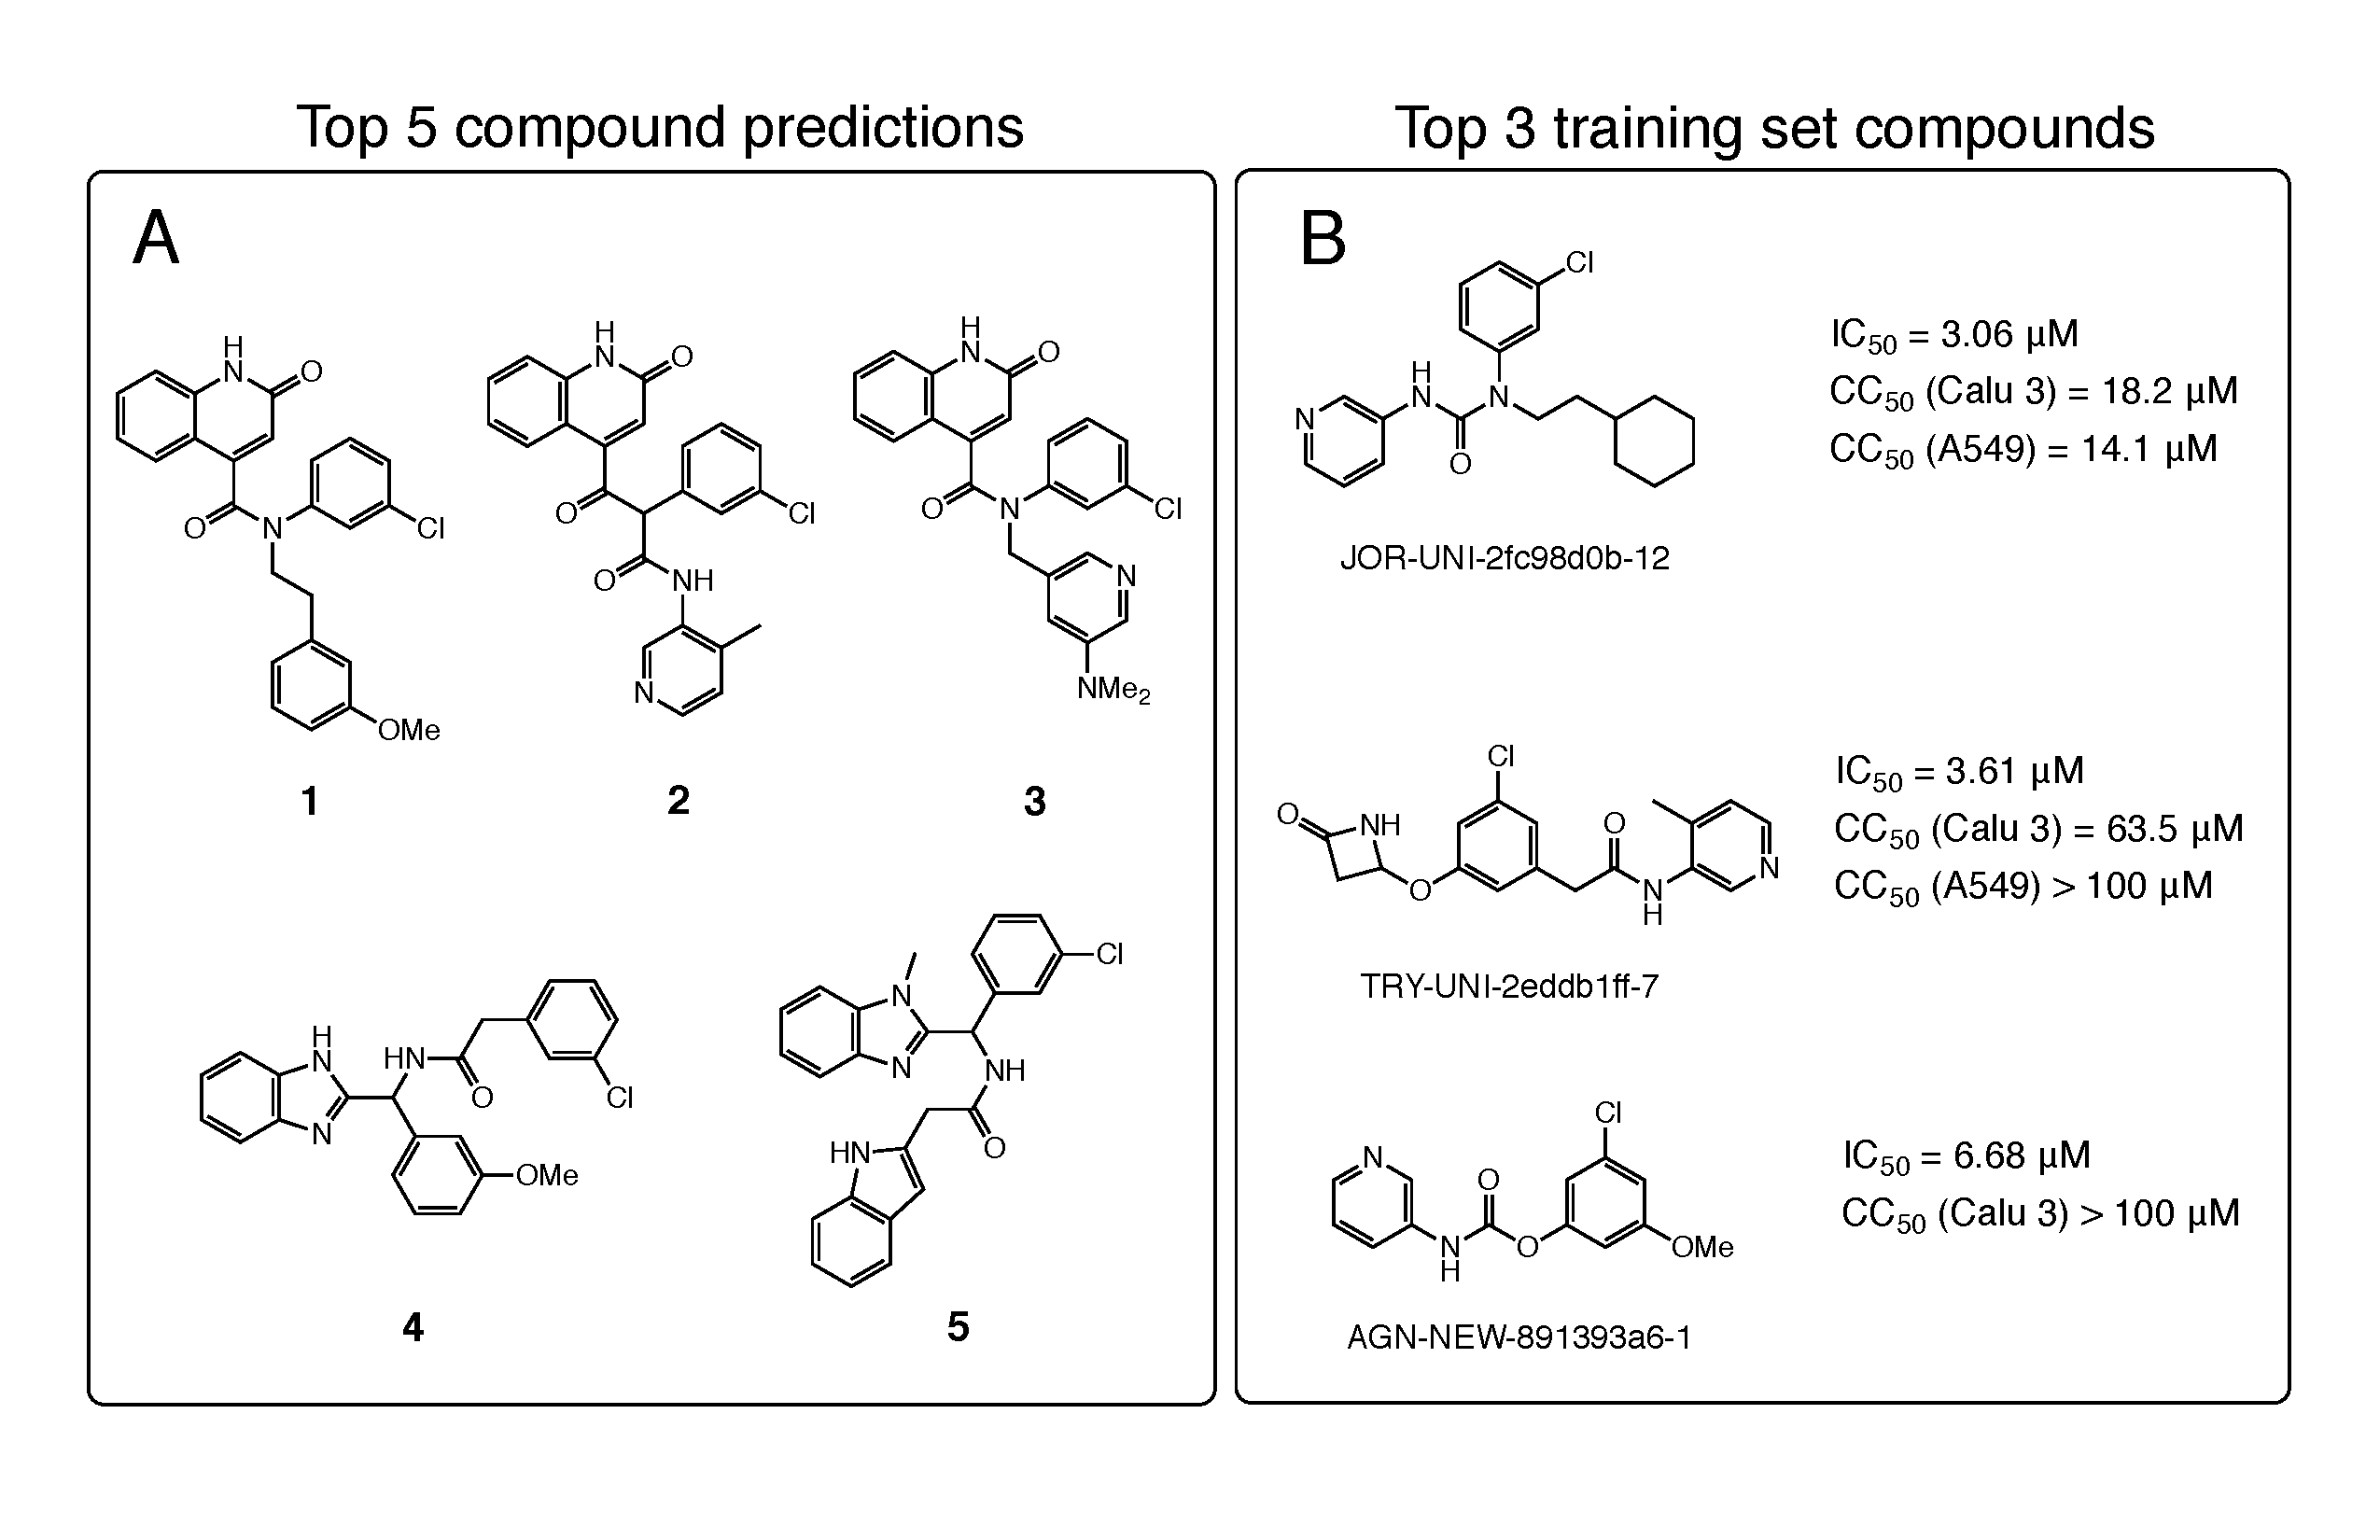
\includegraphics[width=0.45\textwidth]{fig2.pdf}
    \caption{Our synthesis-driven design model prioritises molecular scaffold that are not in the top hits. (A) The 5 compounds selected by our methodology for synthesis and testing. (B) The top 3 compounds from the training set, with potency and cytotoxicity measurements. }
    \label{fig:compounds}
\end{figure}


%describe our generative model + schematic 

Having demonstrated the accuracy of our ranking model, we now turn to chemical space exploration. We first consider a set of chemically reasonable perturbations (e.g. amide to retroamide, amide to urea), which is applied to the whole set of active molecules. We then fragment along synthetically accessible bonds (e.g. amides and aromatic C-C and C-N), and reconnect the synthons to generate an exhaustive library. The resulting library of 8.8 million generated molecules is scored using our ranking model by the probability of having a higher potency compared to the most potent molecule in the dataset.  % We use a simple scheme based on breaking along synthetically accessible bonds. 


\begin{figure}
\centering
         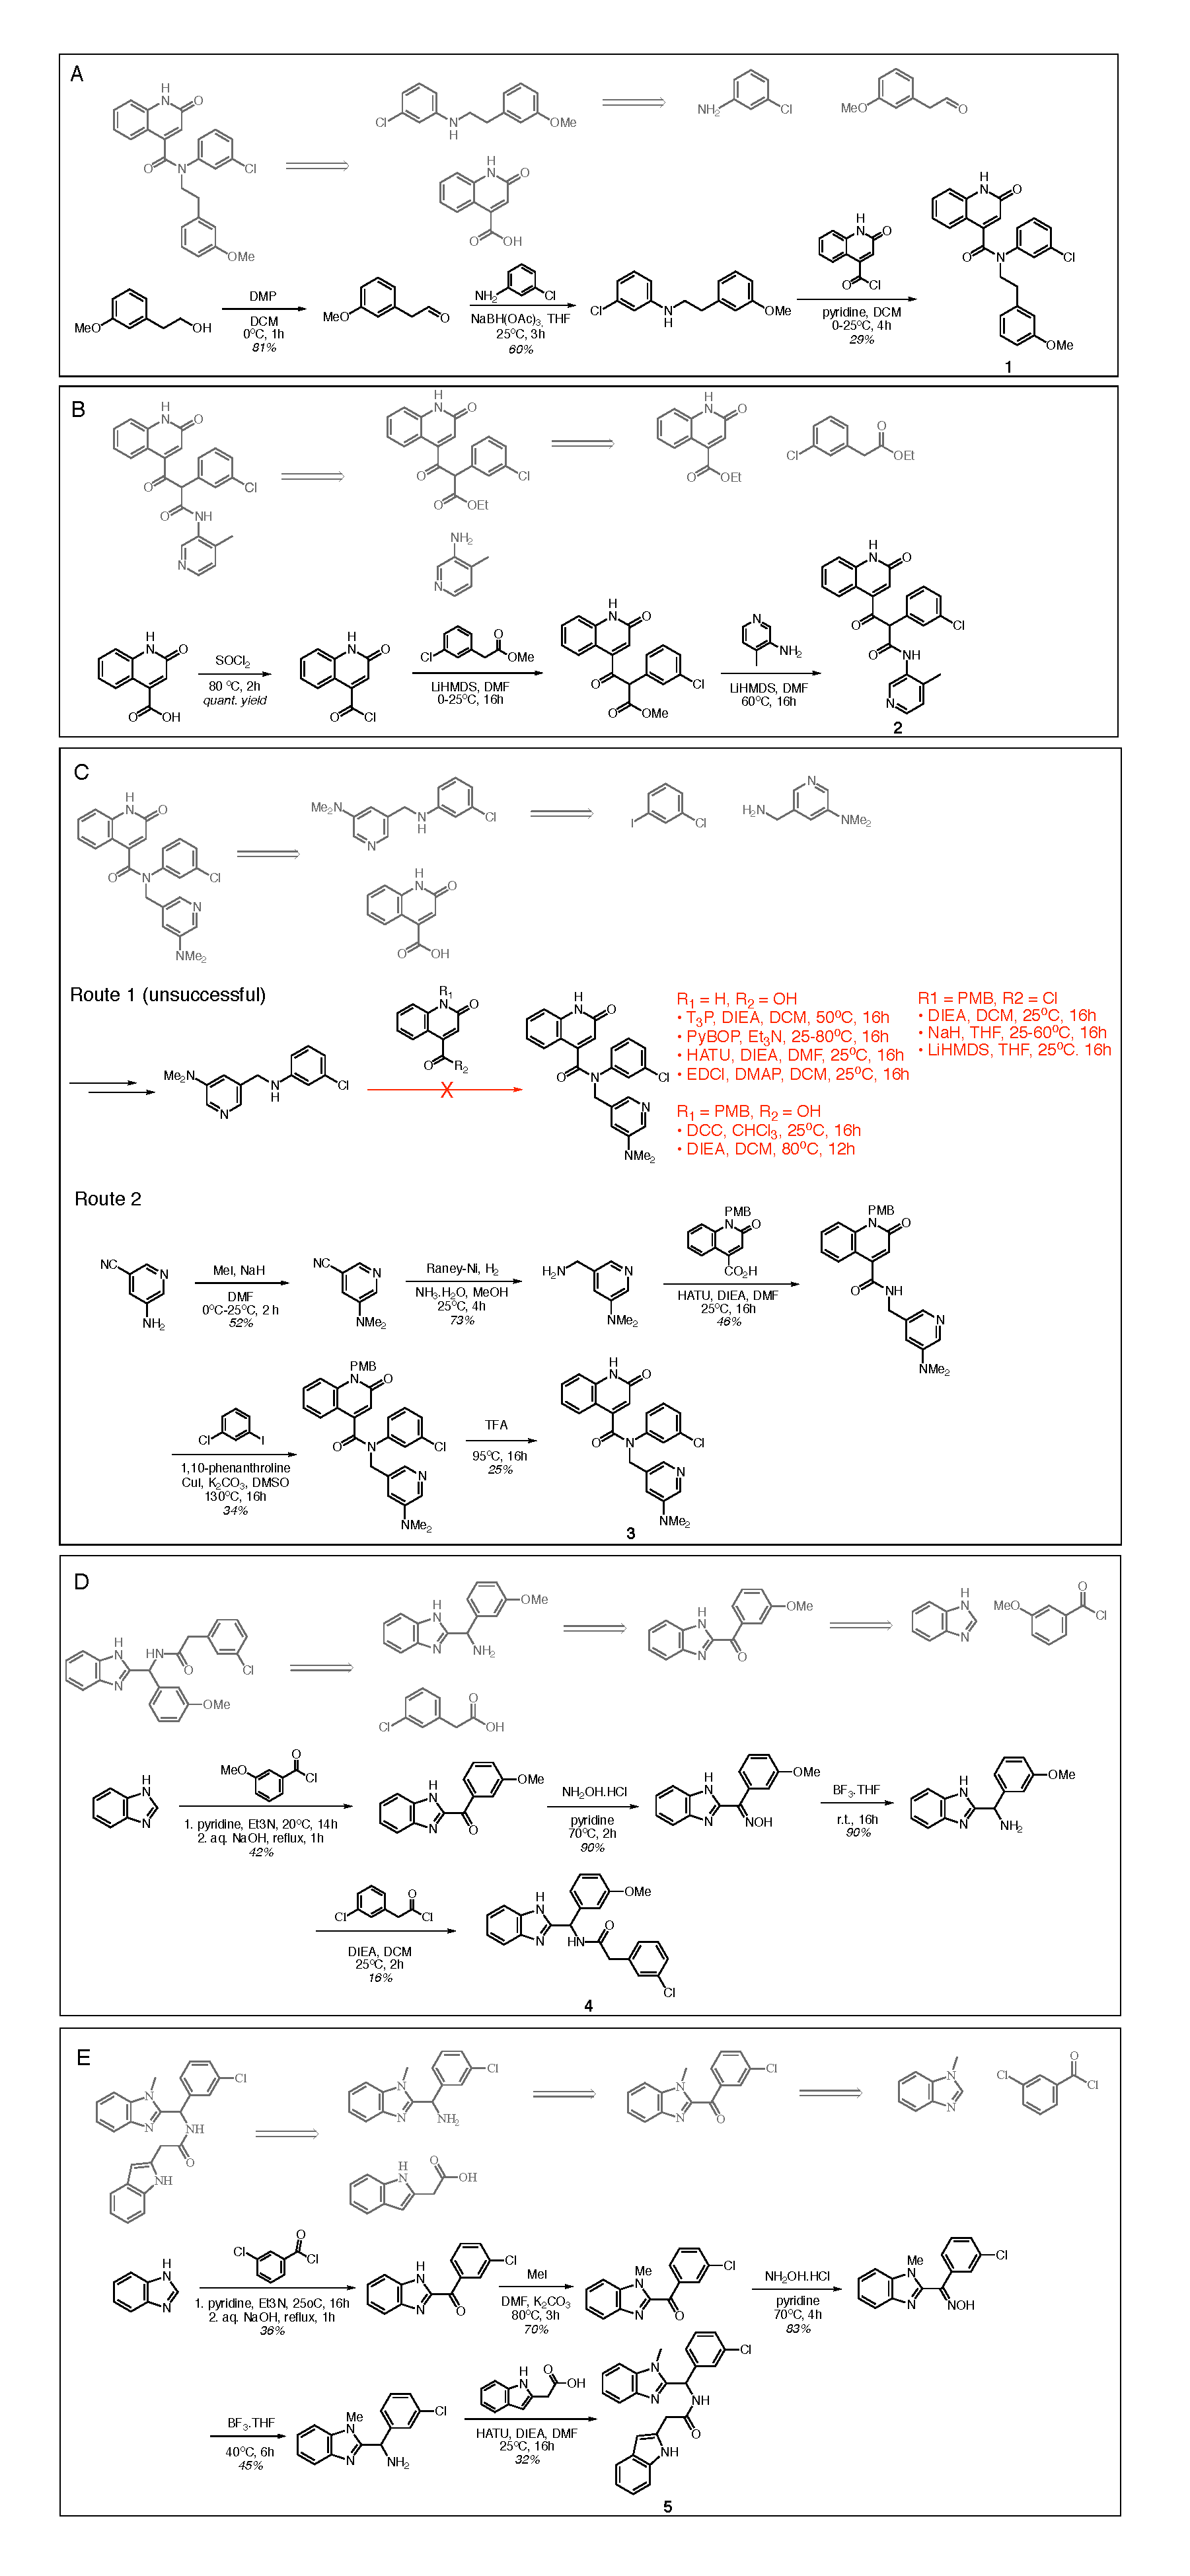
\includegraphics[width=0.5\textwidth]{aaron_schemes.pdf}
    \caption{Model generated synthetic schemes that are experimentally validated. Schemes (A)-(E) show the synthesis schemes generated by our model (grey) and experimental schemes for Compounds $\mathbf{1}$-$\mathbf{5}$. The ESI contains experimental procedures provided by our contract research organisation.}
    \label{fig:synthesis_schemes}
\end{figure}

Although virtual ``reactions'' were used to generate new molecules, the synthons are not necessarily off-the-shelf nor the reactions optimal. As such, we use a retrosynthesis predictor to triage based on synthetic accessibility. We fed top hits into Manifold, our platform for synthesis route prediction (\url{https://postera.ai/manifold}). Manifold searches for synthetic routes starting from purchasable molecules. The underlying technology is based on Molecular Transformer, a machine learning model for reaction prediction using sequence-to-sequence translation \cite{yang2019molecular,schwaller2019molecular}. The top 5 molecules with predicted routes <4 steps were synthesised and tested (Figure \ref{fig:compounds}A). For comparison, the most potent molecules from the training set are shown in Figure \ref{fig:compounds}B; $\mathbf{1}-\mathbf{5}$ have Tanimoto similarity <0.48 (1024-bit ECFP6) to every molecule in the training set. 


Figure \ref{fig:synthesis_schemes} shows that for Compounds $\mathbf{1}$, $\mathbf{2}$, $\mathbf{4}$ and $\mathbf{5}$ our retrosynthesis algorithm generates successful routes, thus provides a reasonable estimate of synthetic complexity. The syntheses were carried out at the Wuxi AppTec and compounds were assayed as received. Minor variations in building blocks were employed depending on what was readily available. We note that our algorithm failed to estimate the synthetic complexity of Compound $\mathbf{3}$. The final amide formation step was unexpectedly challenging, and no desired product was seen despite significant efforts in condition screening. Compound $\mathbf{3}$ was furnished via an alternative strategy, employing an Ullmann coupling to arylate the amide, which was not predicted by our approach. 

%result + discussion 
Compounds $\mathbf{1}$-$\mathbf{5}$ were tested for Mpro activity using a fluorescence assay. Figure \ref{fig:data} shows that Compounds $\mathbf{1}$-$\mathbf{3}$ have $\mathrm{IC}_{50}$ within assay dynamic range ($<100 \mu M$), and Compound $\mathbf{1}$ has $\mathrm{IC}_{50} = 4.1 \mu M$. Compound $\mathbf{1}$ is further assayed in live virus assays, with the less pathogenic OC43 coronavirus, showing $\mathrm{EC}_{50} = 13 \mu M$ and is not cytotoxic ($\mathrm{CC}_{50}>100 \mu M$ against A549 cell line; $CC_{50}$ is the concentration required  to cause 50\% cell death). We employ OC43 as a rapid surrogate assay for SARS-CoV-2 as the former can be done in a BSL-2 rather than BSL-3 lab.  Interestingly, the top non-cytotoxic hit of the training set (TRY-UNI-2eddb1ff-7) does not show OC43 activity, showcasing the utility of using generative models to suggest new scaffolds with complementary physicochemical properties. 

\begin{figure}
\centering
         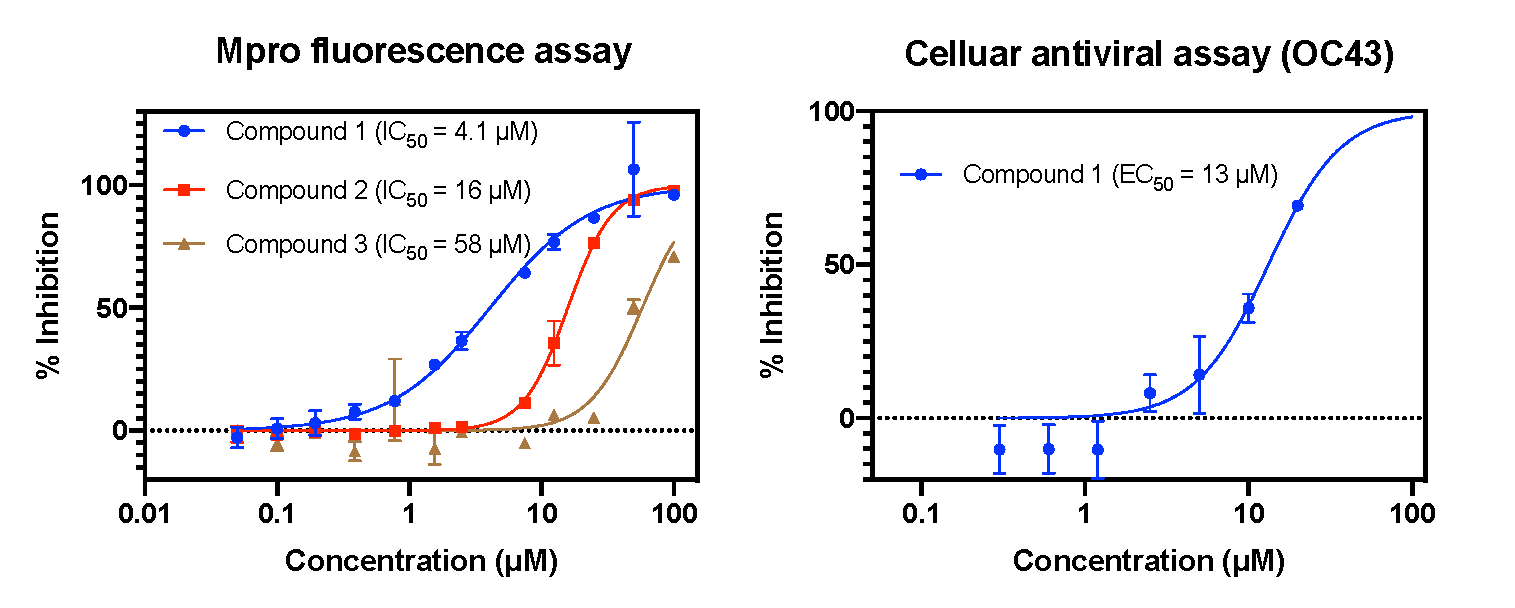
\includegraphics[scale=0.36]{data_curve.pdf}
    \caption{Three compounds generated using our synthesis-directed model exhibit Mpro activity. Our most active compound has measurable antiviral activity against the OC43 coronavirus and no measurable cytotoxic effect ($\mathrm{CC}_{50} (A549)>100 \mu M$). 95\% CI: IC50 (Mpro) -- Compound 1 [3.42,4.86] $\mu$M, Compound 2 [15.1,16.5] $\mu$M, Compound 3 [48.8,69.4] $\mu$M; EC50 (OC43) -- Compound 1 [10.1, 18.4] $\mu$M. See ESI for assay details.}
    \label{fig:data}
\end{figure}

In summary, we demonstrated the utility of a \emph{de novo} design model, guided by estimation of synthetic complexity, for generating ideas in hit expansion. At the time of writing, the quinolone series is undergoing optimisation by the COVID Moonshot initiative (\url{https://postera.ai/covid}). Data for Compound $\mathbf{1}$-$\mathbf{5}$ is registered as the $\texttt{ALP-POS-ddb41b15}$ series on the Moonshot platform. 

%You can also put lists into the text. You can have bulleted or numbered lists of almost any kind. 
%The \texttt{mhchem} package can also be used so that formulae are easy to input: \texttt{\textbackslash ce\{H2SO4\}} gives \ce{H2SO4}. 


%The conclusions section should come at the end of article. For the reference section, the style file \texttt{rsc.bst} can be used to generate the correct reference style.\footnote[4]{Footnotes should appear here. These might include comments relevant to but not central to the matter under discussion, limited experimental and spectral data, and crystallographic data.}

\section*{Acknowledgements}
JDC acknowledges support from NIH grants P30 CA008748 and GM124270. 

\section*{Conflicts of interest}
A.M. and A.A.L are co-founders and shareholders of PostEra (\url{https://postera.ai}). J.D.C is a current member of the Scientific Advisory Board of OpenEye Scientific Software, Interline Therapeutics, and Redesign Science. The Chodera laboratory receives or has received funding from multiple sources,including the National Institutes of Health, the National Science Foundation, the Parker Institute for Cancer Immunotherapy, Relay Therapeutics, Entasis Therapeutics, Silicon Therapeutics, Interline Therapeutics, EMD Serono (Merck KGaA), AstraZeneca, Vir Biotechnology, Bayer, XtalPi, the Molecular Sciences Software Institute, the Starr Cancer Consortium, the Open Force Field Consortium, Cycle for Survival, a Louis V. Gerstner Young Investigator Award, and the Sloan Kettering Institute. A complete funding history for the Chodera lab can be found at \url{http://choderalab.org/funding}.
%%%END OF MAIN TEXT%%%

%  For footnotes in the main text of the article please number the footnotes to avoid duplicate symbols. e.g.  \footnote[num]{your text} the corresponding author \ast counts as footnote 1, ESI as footnote 2, e.g. if there is no ESI, please start at [num]=[2], if ESI is cited in the title please start at [num]=[3] etc. Please also cite the ESI within the main body of the text using \dag.

% The \balance command can be used to balance the columns on the final page if desired. It should be placed anywhere within the first column of the last page.

% \balance

% If notes are included in your references you can change the title from 'References' to 'Notes and references' using the following command:
% \renewcommand\refname{Notes and references}

%%%REFERENCES%%%
\scriptsize{
\bibliography{rsc} %You need to replace "rsc" on this line with the name of your .bib file
\bibliographystyle{rsc} } %the RSC's .bst file

\end{document}
